\documentclass[12pt]{article}
%NOTE TO SELF: BEFORE SUBMITTING MAKE SURE SLL FONTS ARE CORRECT SIZE
\usepackage{graphicx}
%\usepackage{showframe}
\usepackage[top=1.0in, bottom=1.0in, left=1.5in, right=1.0in]{geometry}
\title{A Modern Version Of Space Invaders}
\author{Rian Fitzgerald}
\parindent 0ex
\setlength{\parskip}{1em}
\begin{document}
\pagenumbering{roman}
%\maketitle
\newpage
\begin{center}
\section*{Title}
\end{center}
\newpage
\begin{center}
\section*{Project Summary}
\end{center}
This project is an advanced version of the classic game Space Invaders. It will retain some of the core mechanics and add some features that will provide a challenge for the player. 

There are two parts to this project, the game and the supporting website. The website is used to create accounts for players as well as having a leader board which displays data about the player (for example, their high score, time played and highest level achieved). 

This project uses the same perspective as the original game (top down, two dimensional). The difference between this version and the original is that it will become harder to beat as the players score increases. The objective of the game is to survive as long as possible and achieving the highest score possible. 

This project will use modern tools and techniques as this was a limiting factor in the original implementation. These factors are discussed in more detail in the Background and Research portion of this report. 

\newpage
\begin{center}
\section*{Acknowledgments}
\end{center}
\newpage
\begin{center}
\section*{Declaration}
\end{center}
\newpage

\begin{center}
\tableofcontents
\end{center}

\newpage
\pagenumbering{arabic}



\begin{center}
\section{Introduction}
\end{center}

\begin{center}
\subsection{General Introduction} 
\end{center}
This chapter will give a brief description of the chapters that follow. Chapter two  discusses that background and research that went into this project. Chapter three will show case some of the design that went into this project. Chapter four will address some of the implementation and issues encountered. Chapter five will showcase the testing and evaluation used in the project. The final chapter discusses the conclusions and possible further development of this project.

\begin{center}
\subsection{Motivating Factors}
\end{center}
The main motivation for undertaking this project was to improve the Space Invaders game. From the research completed (this is discussed in Chapter 3), many clones have a set difficulty. This results in an imbalance in the difficulty. A highly skilled player will be able to get a higher score quite easily. The result of this project has created a game that uses information collected by the player to make it more difficult for them to beat. 

A secondary motivation to complete this project was to become familiar with using a modern game engine. It would be a useful skill to add to my repertoire, especially if I want to apply for a job in a game company after college. 

Another motivation for doing this project is to increase my knowledge in web based technologies. As most companies have a web presence it would be useful to know about web technologies, especially those based around JavaScript. 

The final motivation for completing this project is to combine the knowledge I have learned from various modules. This project incorporates aspects of Programming, Object Orientated Programming, Database Systems, Distributed Systems and Systems Analysis and Design. Principles learned from these modules will be applied in the project

\begin{center}
\subsection{Objectives of Proposed Work}
\end{center}
This project has two main objectives with multiple elements to be completed. The two primary objectives are the game and the website. 

The following list details the objectives to be completed for the game.

\begin{enumerate}
\item Programming the initial game using simple graphics.
\item Refining the game mechanics.
\item Program a login screen for the game to allow a player to login so their details can
be recorded.
\end{enumerate}

The next list details the objectives to be completed for the website.

\begin{enumerate}
\item Programming the website.
\item Programming the server.
\item Responding to any GET, POST, PUT and DELETE commands to make the
website RESTful.
\item Creating the database and populate it with test data.
\item Use a testing framework to test if the correct data is being transferred to the
various parts of the project.
\end{enumerate}
\newpage

\begin{center}
\section{Background and Research}
This is some background shite
\end{center}

\begin{center}
\subsection{Analysis of Existing Products}
\end{center}
The original Space Invaders was very primitive in its implementation. It was so primitive that it was unable to render many colours and had to rely on a colour overlay. (arcade-museum.com, 2016). The specification for some of the system is given below


\begin{itemize}
	\item Processor: Intel 8080
	\item Raster graphics on a CRT monitor
	\item Texas Instruments SN76477
\end{itemize}

An interesting point to note is that the graphics were drawn using the processor. This was due to the lack of dedicated graphics processing units at the time. It also explains why the graphics were primitive by today's standards (for example, pixel based with little colouring).

In 1980 a version of Space Invaders was ported to the Atari 2600 (gamespy.com, 2016). This had a number of advantages over the original. The biggest advantage was that the colour palette was increased. Other hardware improvements included the addition of RAM and cartridges that could have memory included. (problemkaputt.de/, 2016)

At the time of writing this report, there are many clones that exist. These clones are available on many platforms from the original game to iOS (kotaku.com, 2016). These clones can differ in many ways from the original. Some will have different aesthetics while others will have different mechanics. The table below is a compiled list of some of the data available about space invaders clones (REFRENCES HERE, 2017).

\begin{center}
    \begin{tabular}{ | p{2.25cm} | p{2.5cm} | p{1.5cm} | p{4cm} |} \hline
    Name & Platform(s) & Released & Features \\ \hline
    Space Invaders (Original) & Arcade, Atari 2600, Nintendo Entertainment System, iOS & 1978, 1980, 1985, 2009 & Raster graphics \\ \hline
    
    Space Invaders Part II, Space Invaders Deluxe (USA) & Arcade, Game Boy & 1979, 1990 & Gameboy version allowed multiplayer, USA version had updated graphics\\ \hline
    
    Space Invaders '95 & Arcade & 1995 & Updated graphics  \\ \hline
    
	Space Invaders 1999, Space Invaders X (Japan) & Playstation, PC, Nintendo 64, Game Boy Color & 1999 & 2D and 3D graphics, competitive mode, cooperative mode,   \\ \hline 
	
	Space Invaders Evolution, Space Invaders: Galaxy Beat (Japan) & Playstation Portable & 2005 & Updated graphics, sounds and gameplay, multiplayer mode, rhythm action gameplay \\ \hline
	
	Space Invaders Extreme & Nintendo DS, Playstation Portable, Xbox 360 & 2008, 2009 & Integrated musical elements \\ \hline
	
	Space Invaders Infinity Gene & iOS, Playstation 3, Xbox 360, Android & 2009, 2010, 2013 & Updated graphics\\ \hline
    \end{tabular}
\end{center}

\newpage
\begin{center}
\subsection{Unity Game Engine}
\end{center}
The Unity engine is a multiplatform game engine. It allows developers to target a range of devices for example PC, Android, iOS and Xbox, to name a few. It uses one click deployment to build solutions for as many devices that are required. (https://unity3d.com/, 2016).

The engine supports a multitude of file formats for images, audio, video and text. The engine abstracts the more difficult aspects of creating a game such as optimisation and graphics rendering. For graphics, it targets APIs depending on which system is selected for the build. Windows can use both Direct3D and OpenGL, Android and iOS use OpenGL ES and consoles use proprietary APIs.

Programming in Unity can be achieved by using a number of languages. The most widely used language for Unity is C#. JavaScript can also be used; however, it is not the same JavaScript that is used for web browsers. It is commonly referred to as UnityScript. (answers.unity3d.com/, 2016). A third language called Boo is also available, however it is now deprecated. It is not documented by Unity anymore, although it will still compile. (forum.unity3d.com, 2016).

Due to its better support and documentation, C# will be the language used to implement the game portion of this project.

\begin{center}
\subsection{MongoDB}
\end{center}
MongoDB is a high performance, scalable, document orientated NoSQL database solution. (stackoverflow.com, 2017). MongoDB uses a JSON-like document with schemas. JSON is a lightweight data format that is easy for humans to read and write as well as to parse for machines. Figure 3.1 shows an example of some data in the JSON format.

JSON is built upon two structures: 
\begin{itemize}
	\item A collection of key/value pairs that correspoind to an abject, record, dictionary, hash table, keyed list or an associative array, depending on which language is being used.
	\item A list of ordered values that correspond to an array, vector or similar data structure. 
\end{itemize}

(json.org, 2017)

\begin{center}
	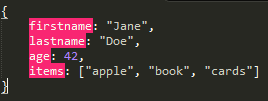
\includegraphics[scale=1]{json_no_id.PNG}
	
	\caption Figure 3.1: Data in JSON format
\end{center}

Because MongoDB is a NoSQL solution the schema is not enforced as strictly as it would in a relational database. The dynamic schema means that each document can have different key/value pairs and can still be inserted into the database. The table shown below summarises the differences between a Relational Database Management System (for example, mySQL) and MongoDB.

\begin{center}
    \begin{tabular}{| l | l |}
    \hline
    Relational Database Management System & MongoDB  \\ \hline
    Table & Collection \\ \hline
    Tuple or Row & Document \\ \hline
    Column & Field \\ \hline
    Primary Key & Key id provided by MongoDB \\ \hline
    \end{tabular}
\end{center}

\begin{center}
\subsection{ExpressJS}
work
\end{center}

\begin{center}
\subsection{AngularJS}
work
\end{center}

\begin{center}
\subsection{NodeJS}
work
\end{center}

\begin{center}
\section{Design}
This is some design shite
\end{center}

\begin{center}
\subsection{Game Design}
work
\end{center}

\begin{center}
\subsection{Database Design}
work
\end{center}

\begin{center}
\subsection{Website Design}
work
\end{center}

\begin{center}
\section{Implementation}
This is some imp shite
\end{center}

\begin{center}
\section{Testing and Evaluation}
This is some testing shite
\end{center}

\begin{center}
\section{Conclusions and Further Development}
This is some imp shite
\end{center}

\begin{center}
\section{Appendicies}
This is some imp shite
\end{center}

\begin{center}
\section{References}
This is some imp shite
\end{center}

\begin{center}
\section{Bibliography}
\end{center}

%\begin{center}
%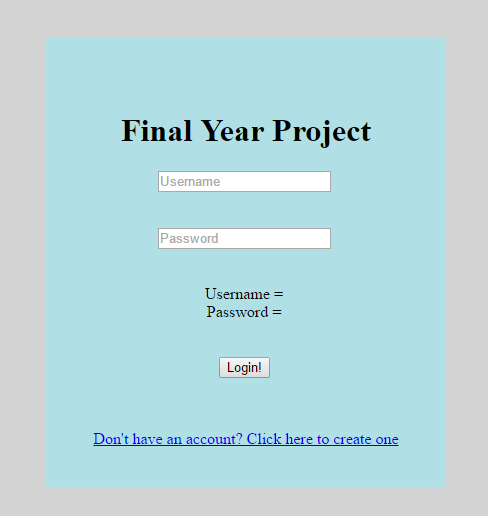
\includegraphics[scale=0.5]{photo.png}
%\end{center}


\end{document}